\section{Modelado}
La fase de modelado es la segunda etapa del proceso de Diseño Guiado por Objetivos (DGO). En esta fase, partiremos de la lista de factoides que
obtuvimos en la etapa anterior y con ella diseñar los prototipos de personas que serán los potenciales usuarios de la misma, representando además
las principales características que extrajimos de los factoides.

Para poder lograr este objetivo, vamos a utilizar el proceso de diseño de personas bottom-up propuesto por Copper, que consta de las siguientes fases:
\begin{itemize}
    \item \textbf{Identificación de variables de comportamiento} $\rightarrow$ El primer paso que vamos a seguir es identificar las distintas variables de comportamiento que vamos a tener en la lista de factoides y ver los posibles valores que van a tomar.
    \item \textbf{Relación de individuos con las variables de comportamiento} $\rightarrow$ Tras haber identificado las variables, vamos a ver para cada uno de los usuarios entrevistados el valor que van a tomar cada una de ellas en base a los factoides obtenidos.
    \item \textbf{Identificación de patrones de comportamiento} $\rightarrow$ Una vez configurada la metriz que relaciona los usuarios con las variables, vamos a marcar en ella las posibles repeticiones que aparezcan para poder establecer un listado de patrones de comportamiento con los que vamos a realizar los esqueletos de las personas.
    \item \textbf{Creación de esqueletos} $\rightarrow$ Tras haber identificado los distintos patrones de comportamiento, vamos a crear los esqueletos que nos van a servir de plantilla para las personas definitivas que vamos a desarrollar en los siguientes apartados.
    \item \textbf{Revisión de la completitud y la redundancia} $\rightarrow$ Cuando los esqueletos de las personas ya estén finalizados, el siguiente paso es comprobar su completitud y evitar posibles redundancias entre ellos, haciendo que todas las personas que se representen tengan todos los factoides y se eviten repeticiones entre ellas.
    \item \textbf{Elaboración de las personas} $\rightarrow$ Al finalizar la revisión de los esqueletos, lo siguiente que ha de hacerse es desarrollar las personas a partir de ellos, dando los principales motivos y acciones que llevan a cada una de ellas.
    \item \textbf{Validación de las personas} $\rightarrow$ Para poder validar las personas, tenemos que cerciorarnos de que representen todos y cada uno de los factoides que tenemos, tanto los de las entrevistas como los de los cuestionarios y el análisis de la competencia.
    \item \textbf{Tipos de las personas} $\rightarrow$ Por último, cuando ya se tienen validadas todas las personas elaboradas, vamos a decir en base a las características que presentan, el tipo de persona ante el que nos encontramos.
\end{itemize}

\subsection{Planificación del hito}
Para poder planificar este hito correctamente, hemos identificado en una Hoja de cálculo (ver figura \ref{fig:planif-hito2}) las distintas tareas que tenemos que 
realizar, junto al intervalo de fechas en el que se encuentra prevista su realización y el / los responsables de dicha tarea.

\begin{figure}[H]
    \centering 
    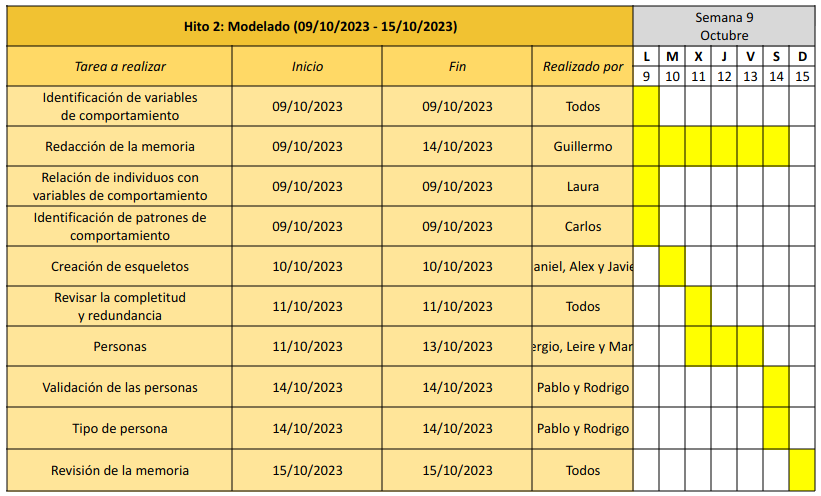
\includegraphics[width=0.5\textwidth]{./Imagenes/Planificaciones/Planif-hito2.png}
    \caption{Planificación Hito 2}
    \label{fig:planif-hito2}
\end{figure}

\subsection{Identificación de variables de comportamiento}
En la fase de modelado, el primer paso que debemos seguir es la identificación de las variables de comportamiento. Estas variables van a ser producto de las listas de factoides que confeccionamos durante el hito anterior y hemos corregido antes de comenzar a trabajar en este. El proceso de confección de las variables consiste en identificar posibles características que pueden encasillar a los usuarios y a partir de ellas darles un rango de valores que podamos asignar a nuestros usuarios. Para reflejar estas variables, hemos construido una tabla (ver cuadro \ref{table:variables-comportamiento}) en la que podemos observarlas junto a los valores que pueden tomar.
\begin{table}[h]
    \centering
    \begin{tabular}{|c|c|}
        \hline
        \textbf{Variable} & \textbf{Posibles valores} \\ \hline
        Rango de Edad & 18- / 18 - 25 / 26 - 40 / 40 - 65 / 65+ \\ \hline
        Estado civil & Casad@ / En pareja / Solter@ \\ \hline
        Organización de viajes & Sí / No \\ \hline
        Uso de comparadores de viajes & Sí / No (Si los usa especificar cuáles) \\ \hline
        Frecuencia de viaje & Baja / Media / Alta \\ \hline
        Tipo de viaje & Ocio / Trabajo / Estudios \\ \hline
        Discapacidad & Sí / No / Acompañante \\ \hline
        Acompañante & Familia / Amigos / Pareja / Solo \\ \hline
        Medio de transporte más frecuente & Avión / Tren / Vehículo propio / Transporte público / Otro \\ \hline
        Uso de tecnología & Básica / Avanzada \\ \hline
        Viaje nacional & Sí / No \\ \hline
        Viaje internacional & Sí / No \\ \hline
        Trabaja & Sí / No \\ \hline
        Gusto por viajar & Sí / No \\ \hline
        Nivel de ahorro & Bajo / Medio / Alto \\ \hline
    \end{tabular}
    \caption{Variables de comportamiento y sus valores}
    \label{table:variables-comportamiento}
\end{table}
\subsection{Relación de individuos con variables de comportamiento}
Tras haber identificado las variables de comportamiento en la fase anterior, vamos a ver para cada uno de los usuarios entrevistados (en base a los factoides
que tenemos registrados) los valores que van a tomar en cada una de ellas. Para mostrar estos resultados vamos a realizar una matriz (ver cuadro \ref{table:relacion-individuos-variables})
en la que vamos a enfrentar cada una de las variables con los entrevistados, poniendo en cada celda el valor que va a tomar la variable para dicho usuario.
\begin{table}[H]
    \centering
    \begin{tabular}{|p{10em}|p{7em}|p{7em}|p{7em}|p{8em}|}
        \hline
        \cellcolor{black}                 & \cellcolor{black}{\textcolor{white}{Madi}}  & \cellcolor{black}{\textcolor{white}{Sofía}}   & \cellcolor{black}{\textcolor{white}{Beatriz}} \\ \hline
        Rango de edad                     &                                             & 18 - 25                                       & 18 - 25                                       \\ \hline
        Estado civil                      &                                             & Soltera                                       & En pareja                                     \\ \hline
        Organización de viajes            & Si                                          & Si                                            & Si                                            \\ \hline
        Uso de comparadores de viajes     & No                                          & Kayak, Skyscanner, Trivago                    & eDreams, comparador de Google                 \\ \hline
        Frecuencia de viaje               & Alta                                        & Media                                         & Baja                                          \\ \hline
        Tipo de viaje                     & Trabajo                                     & Ocio                                          & Ocio                                          \\ \hline
        Discapacidad                      & No                                          & No                                            & No                                            \\ \hline
        Acompañante                       &                                             & Familia                                       & Familia                                       \\ \hline
        Medio de transporte más frecuente &                                             & Transporte público                            & Vehículo propio                               \\ \hline
        Uso de tecnología                 &                                             & Alto                                          & Alto                                          \\ \hline
        Viaje nacional                    & Si                                          & Si                                            & Si                                            \\ \hline
        Viaje internacional               & Si                                          & Si                                            & Si                                            \\ \hline
        Trabaja                           & Si                                          & No                                            & No                                            \\ \hline
        Gusto por viajar                  &                                             & Si                                            & Si                                            \\ \hline
        Nivel de ahorro                   & Alto                                        & Alto                                          & Alto                                          \\ \hline
    \end{tabular}
    \caption{Matriz de relación de los individuos con las variables de comportamiento}
    \label{table:relacion-individuos-variables}
\end{table}

Una vez construida la matriz que relaciona los individuos con las variables, vamos a justificar las razones por las cuáles hemos asignado un
determinado valor a las variables para cada uno de los usuarios. \\

\noindent Justificación de las variables de Madi:
\begin{itemize}
    \item \textbf{Rango de edad} $\rightarrow$ No lo ha comentado.
    \item \textbf{Estado civil} $\rightarrow$ No lo ha comentado.
    \item \textbf{Organización de viajes} (Si) $\rightarrow$ “Madi se encarga de organizar los viajes cuadrando horarios y comprando billetes.”
    \item \textbf{Uso de comparadores de viajes} (No) $\rightarrow$ “Madi no utiliza comparadores porque ya tiene localizadas dos compañías y Renfe que ofrecen el servicio de acompañamiento de AENA.”
    \item \textbf{Frecuencia de viaje} (Alta) $\rightarrow$ “Madi se encarga de los viajes de campeonatos internacionales que ella les recepciona, les recoge y les lleva al punto de encuentro. Madi comenta que hay bastantes campeonatos.” Porque al menos asiste a los viajes internacionales que pueden ser no muy frecuentes.
    \item \textbf{Tipo de viaje} (Trabajo) $\rightarrow$ Se encarga de los viajes de su trabajo y viaja por ello.
    \item \textbf{Discapacidad} (No) $\rightarrow$ Se deduce porque trabaja en una federación y organiza viajes para gente con discapacidad.
    \item \textbf{Acompañante} $\rightarrow$ No lo ha comentado, podría ser sus compañeros de trabajo.
    \item \textbf{Medio de transporte más frecuente} $\rightarrow$ no se sabe realmente, podría ser avión o tren.
    \item \textbf{Uso de la tecnología} $\rightarrow$ tampoco lo comenta, sólo el de los deportistas.
    \item \textbf{Viaje Nacional} (Si) $\rightarrow$ “Madi comenta que en los campeonatos de españa, los clubes son los encargados del desplazamiento de los deportistas, ella interviene poco o nada.” eso significa que el poco puede llegar a viajar en algún momento en los nacionales.
    \item \textbf{Viaje internacional} (Si) $\rightarrow$ “Madi se encarga de los viajes de campeonatos internacionales que ella les recepciona, les recoge y les lleva al punto de encuentro. Madi comenta que hay bastantes campeonatos.”, recoge a los deportistas por lo que hace el viaje.
    \item \textbf{Trabaja} (Si) $\rightarrow$ “Madi es secretaria de la FEDDI y lleva 16 años trabajando allí.”
    \item \textbf{Gusto por viajar} $\rightarrow$ No lo ha dicho.
    \item \textbf{Nivel de Ahorro} (Alto) $\rightarrow$ “Madi compra billetes a través de Renfe, Air Europa o Iberia porque le sale más económico que en un comparador.” suponemos que escoge lo más económico para ahorrar lo máximo posible.
\end{itemize}

\noindent Justificación de las variables de Sofía:
\begin{itemize}
    \item \textbf{Rango de edad} (18 - 25) $\rightarrow$ “Sofía tiene 21 años.”
    \item \textbf{Estado civil} (Soltero) $\rightarrow$ No lo ha comentado, pero parece no tener pareja. 
    \item \textbf{Organización de viajes} (Si) $\rightarrow$ “Sofía a veces organiza los viajes que hace y a veces no.”
    \item \textbf{Uso de comparadores de viajes} (Kayak, Skyscanner, Trivago) $\rightarrow$ “Sofía utiliza varios comparadores de viajes a la hora de organizar un viaje. Por ejemplo: Kayak, Skyscanner, Trivago.”
    \item \textbf{Frecuencia de viaje} (Media) $\rightarrow$ “Sofía viaja a menudo, tanto fuera como dentro de España.”, a menudo será lo normal.
    \item \textbf{Tipo de viaje} (Ocio) $\rightarrow$ “Sofía ha hecho viajes de varios tipos. Desde intercambios lingüísticos a viajes familiares o con amigos, para conocer nuevas ciudades o relajarse.”
    \item \textbf{Discapacidad} (No) $\rightarrow$ “Sofía considera que los comparadores de viajes son bastante accesibles, pero que quizás aclarar algunas cosas en las webs o los anuncios de spam en las webs pueden molestar a personas con discapacidad intelectual.” da a intuir que ella no tiene discapacidad.
    \item \textbf{Acompañante} (Familia) $\rightarrow$ “A Sofía le gusta ir alternando entre viajar sola, con familia o con amigos, disfruta de todas.” Más con familia ya que es estudiante y no tiene trabajo para pagar tantos viajes.
    \item \textbf{Medio de transporte más frecuente} (Transporte público) $\rightarrow$ “Sofía usa tanto automóviles como trenes y autobuses en sus viajes dependiendo del sitio al que viaje.” “Sofía prefiere usar autobuses solo cuando viaje distancias cortas o medias” En cualquiera de los dos casos incluye transporte público.
    \item \textbf{Uso de la tecnología} (Alto) $\rightarrow$ “Sofía tiene 21 años y considera que tiene un buen manejo de la tecnología”
    \item \textbf{Viaje Nacional} (Si) $\rightarrow$ “Sofía viaja a menudo, tanto fuera como dentro de España.”
    \item \textbf{Viaje internacional} (Si) $\rightarrow$ “Sofía viaja a menudo, tanto fuera como dentro de España.”
    \item \textbf{Trabaja} (No) $\rightarrow$ “Sofía es estudiante, tiene 21 años y considera que tiene un buen manejo de la tecnología” 
    \item \textbf{Gusto por viajar} (Si) $\rightarrow$ “A Sofía le gusta viajar y desde pequeña ha querido conocer las diferentes partes del mundo.”
    \item \textbf{Nivel de Ahorro} (Alto) $\rightarrow$ “Sofía busca viajes económicamente accesibles.” quiere ahorrar lo máximo posible.
\end{itemize}

\noindent Justificación de las variables de Beatriz:
\begin{itemize}
    \item \textbf{Rango de edad} (18 - 25) $\rightarrow$ “Beatriz tiene 21 años.”
    \item \textbf{Estado civil} (En pareja) $\rightarrow$ "Va a viajar a ver a su pareja en los próximos meses".
    \item \textbf{Organización de viajes} (Si) $\rightarrow$ “Cuando no viaja con su familia, Beatriz suele organizar los viajes que hace. Cuando va con su familia, lo organiza todo el núcleo familiar en conjunto”.
    \item \textbf{Uso de comparadores de viajes} (eDreams, comparador de Google)
    \item \textbf{Frecuencia de viaje} (Baja) $\rightarrow$ “Beatriz viaja una vez al año, sobre todo dentro de España, y fuera de España una vez cada dos años.” es poco
    \item \textbf{Tipo de viaje} (Ocio) $\rightarrow$ “Beatriz suele viajar para visitar a familiares o por razones de ocio.”
    \item \textbf{Discapacidad} $\rightarrow$ No lo dice en ningún momento.
    \item \textbf{Acompañante} (Familia) $\rightarrow$ “Beatriz suele viajar acompañada, mayoritariamente por algún familiar suyo”.
    \item \textbf{Medio de transporte más frecuente} (Vehículo propio) $\rightarrow$ “Suele viajar en coche o en avión para distancias más largas.” como es dentro de España lo más normal, viaja en vehículo propio más frecuentemente.
    \item \textbf{Uso de la tecnología} (Alto) $\rightarrow$ “Beatriz se desenvuelve bien con las tecnologías y declara usarlas a diario.”
    \item \textbf{Viaje Nacional} (Si) $\rightarrow$ “Beatriz viaja una vez al año, sobre todo dentro de España, y fuera de España una vez cada dos años.”
    \item \textbf{Viaje internacional} (Si) $\rightarrow$ “Beatriz viaja una vez al año, sobre todo dentro de España, y fuera de España una vez cada dos años.”
    \item \textbf{Trabaja} $\rightarrow$ No lo comenta
    \item \textbf{Gusto por viajar} (Si) $\rightarrow$ “A Beatriz le gusta viajar para conocer otros lugares y culturas.”
    \item \textbf{Nivel de Ahorro} (Alto) $\rightarrow$ “Para Beatriz no es ningún problema sacrificar algunas facilidades como el  tipo y la cantidad de equipaje que se puede llevar, el hecho de elegir asiento o los horarios de ida y vuelta porque cuanto más barato mejor.”
\end{itemize}

\subsection{Identificación de patrones de comportamiento}
Para identificar los patrones de comportamiento nos hemos basado en la comparación de los usuarios y buscar similitudes en sus gustos a raíz de las variables de comportamiento previamente estudiadas (ver cuadro \ref{table:relacion-individuos-variables-patrones}).
\begin{table}[H]
    \centering
    \begin{tabular}{|p{10em}|p{7em}|p{7em}|p{7em}|p{8em}|}
        \cellcolor{black}                 & \cellcolor{black}{\textcolor{white}{Madi}}  & \cellcolor{black}{\textcolor{white}{Sofía}}   & \cellcolor{black}{\textcolor{white}{Beatriz}}     \\ \hline
        Rango de edad                     &                                             & \cellcolor{green}{18 - 25}                    & \cellcolor{green}{18 - 25}                        \\ \hline
        Estado civil                      &                                             & Soltera                                       & En pareja                                         \\ \hline
        Organización de viajes            & Si                                          & \cellcolor{green}{Si}                         & \cellcolor{green}{Si}                             \\ \hline
        Uso de comparadores de viajes     & \cellcolor{yellow}{No}                      & \cellcolor{purple}{Kayak, Skyscanner, Trivago}& \cellcolor{purple}{eDreams, comparador de Google} \\ \hline
        Frecuencia de viaje               & \cellcolor{yellow}{Alta}                    & \cellcolor{purple}{Media}                     & \cellcolor{purple}{Baja}                          \\ \hline
        Tipo de viaje                     & Trabajo                                     & \cellcolor{green}{Ocio}                       & \cellcolor{green}{Ocio}                           \\ \hline
        Discapacidad                      & No                                          & \cellcolor{green}{No}                         &                                                   \\ \hline
        Acompañante                       &                                             & \cellcolor{blue}{Familia}                     & \cellcolor{blue}{Familia}                         \\ \hline
        Medio de transporte más frecuente &                                             & Transporte público                            & Vehículo propio                                   \\ \hline
        Uso de tecnología                 &                                             & \cellcolor{green}{Alto}                       & \cellcolor{green}{Alto}                           \\ \hline
        Viaje nacional                    & \cellcolor{orange}{Si}                      & \cellcolor{orange}{Si}                        & \cellcolor{orange}{Si}                            \\ \hline
        Viaje internacional               & \cellcolor{orange}{Si}                      & \cellcolor{orange}{Si}                        & \cellcolor{orange}{Si}                            \\ \hline
        Trabaja                           & \cellcolor{yellow}{Si}                      & No                                            &                                                   \\ \hline
        Gusto por viajar                  &                                             & \cellcolor{green}{Si}                         & \cellcolor{green}{Si}                             \\ \hline
        Nivel de ahorro                   & Alto                                        & \cellcolor{purple}{Alto}                      & \cellcolor{purple}{Alto}                          \\ \hline
    \end{tabular}
    \caption{Matriz de la relación de los individuos con las variables de comportamiento (patrones)}
    \label{table:relacion-individuos-variables-patrones}
\end{table}
Tras realizar el análisis de la matriz anterior hemos identificado los siguientes patrones de comportamiento:
\begin{itemize}
    \item La gente entre 18 y 25 años comparte un gusto por viajar (sobre todo viajes de ocio), tiene un alto uso de la tecnología y tienen un nivel de ahorro alto.
    \item La mitad de las personas utilizan comparadores para organizar los viajes.
    \item La mitad de la gente entrevistada viaja con sus familiares.
    \item A casi todos los entrevistados les gustan los viajes internacionales.
    \item En general la frecuencia de viajes de los usuarios son media-bajas.
    \item Las personas que están solteras viajan con sus familiares.
    \item Las personas que trabajan tienen una frecuencia de viajes alta.
    \item Las personas que no trabajan tienen una frecuencia de viajes media-baja.
    \item Las personas que viajan menos utilizan comparadores de viajes y tienen un nivel de ahorro alto.
    
\end{itemize}

Tras finalizar este proceso de identificación de los patrones de comportamiento, vamos a concluir que tenemos tres tipos de personas. El primero de ellos se trata de personas (normalmente jóvenes) a los que les gusta viajar y se organizan sus propios viajes usando comparadores. El segundo tipo de persona que vamos a tener va a ser personas que tengan un trabajo, que viajan por trabajo y que no organizan sus viajes. Por último, vamos a tener personas con discapacidad (física e intelectual), que desisten al usar los comparadores.

\subsection{Creación de esqueletos}
En el apartado anterior identificamos (de forma descriptiva) los distintos tipos de personas que vamos a tener. El siguiente paso va a ser elaborar el esqueleto de dichas personas, para lo cuál se han seguido los siguientes pasos. En primer lugar se han consultado las distintas listas de factoides y los patrones de comportamiento que se han identificado para ver los tres tipos de usuarios diferenciados que tenemos. Posteriormente se han añadido los factoides identificados en los cuestionarios analizando las estadísticas de estos. A continuación pueden verse los resultados del proceso. \\

\noindent \textbf{Viajante que usa comparadores de viajes}
\begin{itemize}
    \item Marta González Torres
    \item 23 años.
    \item Viven en ciudad.
    \item Estudiante.
    \item Gusto por viajar para conocer nuevas culturas (ocio).
    \item Prefiere buscar en el ordenador.
    \item Tiene un uso alto de la tecnología.
    \item Tiene una frecuencia de viaje media alta.
    \item Persona soltera
    \item Viaja en familia
    \item Utiliza Trivago, SkyScanner, eDreams o busca en las páginas de las aerolíneas.
    \item Objetivos:
    \begin{itemize}
        \item Ahorrar la mayor cantidad de dinero posible al realizar el viaje.
        \item Poder asistir a eventos cuando viaja (sobre todo musicales).
        \item Realizar viajes tanto nacionales como internacionales.
        \item Encontrar el mejor vuelo horario-precio.
    \end{itemize}         
\end{itemize}

\noindent \textbf{Viajante que no usa comparadores de viajes (de forma habitual)}
\begin{itemize}
    \item Juan Martínez Díaz
    \item 24 años
    \item Vive en ciudad
    \item Trabaja
    \item Le gusta viajar
    \item Está en pareja
    \item Viaja por trabajo
    \item Tiene una frecuencia de viaje media y le gustaría viajar más.
    \item Tiene un uso alto de la tecnología 
    \item En distancias cortas se desplaza en autobús.
    \item Objetivos:
    \begin{itemize}
        \item Intentar mantener un nivel de ahorro medio.
        \item Poder realizar viajes tanto nacionales como internacionales
    \end{itemize}                      
\end{itemize}

\noindent \textbf{Viajante con discapacidad}
\begin{itemize}
    \item Isabel García Rodríguez
    \item 30 años
    \item Vive en ciudad
    \item Persona con discapacidad física
    \item Planifica sus viajes
    \item Puede encontrar alguna dificultad a la hora de hacer búsquedas (necesita medios accesibles).
    \item Conoce de antemano las empresas que le pueden proporcionar servicios accesibles para ella.
    \item A veces necesita de un acompañante que la ayude a desplazarse.
    \item Viaja para ver a sus familiares.
    \item Objetivos:
    \begin{itemize}
        \item Poder realizar sus viajes buscando medios de transporte accesibles.
        \item No tiene problemas para comprender la página, pero entiende que hay usuarios a los que sí les puede costar.
        \item Le parece complicado pedir ayuda dentro de los comparadores de viajes.
    \end{itemize}             
\end{itemize}

\subsection{Revisar la completitud y la redundancia}
En esta fase, el objetivo principal es tomar los esqueletos que se han generado en la etapa anterior y comprobar que se encuentran acordes a la lista de factoides y que además no son redundantes entre sí. Para ello, se han comprobado de manera individual los factoides, las variables de comportamiento y los patrones de comportamiento detectados para crear los esqueletos y en cuanto a completitud todo está reflejado en ellos. 
Hay una diferencia clara entre los viajantes que utilizan comparadores y los que no y las personas con discapacidad. 
En cuanto a la redundancia hemos comprobado que no es posible fusionar los esqueletos, ya que, con todas las características presentes, no tienen atributos en común que lo permitan. Por ello, comenzaremos a desarrollar las personas que finalmente van a ser el resultado de este hito.

\subsection{Personas}
Tras haber revisado la completitud y la redundancia de los esqueletos que hemos generado, vamos a elaborar las distintas personas a partir de ellos, garantizando que mantienen todas las características que se han pensado para ellos y que contienen todos los elementos de la lista de factoides. \\

Para configurar estas personas, hemos utilizado un formato en el que vamos a dar en primer lugar la información general de la persona (edad, sexo, estudios y gustos). Posteriormente vamos a poner una foto de la persona (generada por una inteligencia artificial) y por último una descripción más elaborada de la persona, conteniendo la gran mayoría de los factoides e ideas expresadas en los esqueletos de las personas. Para poder destacar estas ideas, las hemos puesto en cursiva. \\

La estructura que van a tener las distintas personas va a tener la siguiente configuración (ver figura \ref{fig:estructura-personas}) con los contenidos que hemos mecionado anteriormente.
\begin{figure}[h]
    \centering
    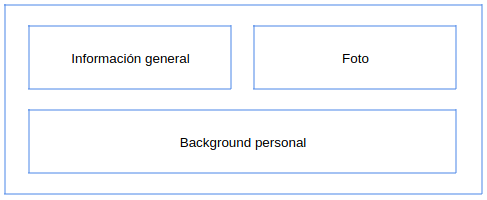
\includegraphics[width=0.5\textwidth]{Imagenes/Personas/Plantilla personas.png}
    \caption{Estructura de las personas}
    \label{fig:estructura-personas}
\end{figure}

\subsubsection{Marta González Torres}

\begin{minipage}{0.4\textwidth}
    \textbf{Información general} \\

    Edad: \textit{23 años} \\
    Sexo: Mujer \\
    Estudios: Ingeniería de Telecomunicaciones \\
    Gustos: Escuchar música e ir a conciertos cuando puede \\
\end{minipage}
\hfill
\begin{minipage}{0.4\textwidth}
    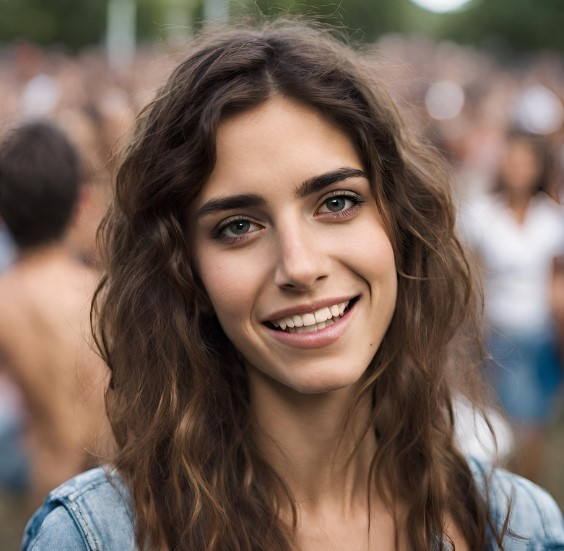
\includegraphics[width=0.5\textwidth]{Imagenes/Personas/Marta.jpg}
\end{minipage}

\textbf{Background personal} \\

Marta no puede salir de su casa sin los auriculares. Para ella la música es una gran parte
de su vida, y todas las mañanas, en la parada del bus, \textit{se prepara un playlist personalizada
en Spotify} para el itinerario hasta la Universidad. \textit{Vive en Fuenlabrada}, por lo que tiene
una ruta de una hora hasta que llega a Madrid, \textit{donde va a clase en la UCM}. \\ 

A Marta sobre todo le gusta la música italiana, ya que en el 2020 se fue de Erasmus a Turín y se
enamoró tanto de su cultura como de su música. Su cantante favorita es Francesca Michielin, así que
cuando hace gira intenta ir a algún concierto suyo en una \textit{ciudad italiana en la que no haya
estado}. De esta manera, puede conocer más la cultura italiana que tanto le gusta y sus diferenciados
a lo largo del país. \\

Se da la casualidad de que a su hermano Julián también le gusta mucho Francesca, así que en varias
ocasiones \textit{han ido ellos de viaje junto a sus padres} Carlos y Elena, los cuáles se van a
cenar juntos mientras sus hijos están en el concierto. \textit{Esto no lo hacen muy a menudo} debido
a que solo van cuando hay un concierto en alguna ciudad que les resulte interesante a toda la familia.
Normalmente se encarga ella de hacer la reserva tanto de los vuelos, \textit{para lo que usa
SkyScanner, como del alojamiento, utilizando AirBnB en este caso}. Esto se le hace a veces complicado
ya que quieren ir a varios sitios y tiene que cuadrar los horarios de todo. Por este motivo prefiere usar la 
aplicación web de las compañías, ya que así puede tener varias pestañas abiertas en las que visualiza toda
la información a la vez. \\

Con respecto al tema universitario, a Marta se le está haciendo cuesta arriba. Se metió inicialmente
en telecomunicaciones porque \textit{se le daban bien las matemáticas y la tecnología}, pero la
carrera no fue lo esperado. A pesar de las dificultades, la carrera le gusta y querría terminarla,
ya que este será en principio su último año. Pero estos problemas la agobian bastante, y para
distraerse le gusta mucho \textit{ir a festivales de música por España}. Suele ir todos los años
al festival Starlite, pues Pablo, el novio de su hermano y con el que mantiene muy buena relación,
es de Marbella, y se puede quedar algunos días en la playa aprovechando el viaje. Pero a pesar de
que no tiene que pagar gastos de alojamiento, el evento musical es bastante caro (ya que va varios
días), por lo que \textit{intenta ahorrar lo máximo posible en el viaje}. Para eso usa comparadores
de viaje como Omio, además de revisar las páginas de aerolíneas como \textit{RyanAir}, ya que a veces son
incluso más baratas que un vuelo o un tren.

\subsubsection{Juan Martínez Díaz}

\begin{minipage}{0.4\textwidth}
    \textbf{Información general} \\

    Edad: \textit{24 años} \\
    Sexo: Hombre \\
    Estudios: Derecho \\
    Gustos: Ir al gimnasio y compartir tiempo con sus amigos. \\
\end{minipage}
\hfill
\begin{minipage}{0.4\textwidth}
    
\includegraphics[width=0.5\textwidth]{Imagenes/Personas/Juan.jpg}
\end{minipage}

\textbf{Background personal} \\

Juan es una persona muy extrovertida y activa, siempre buscando nuevos retos y experiencias. Es por eso por lo que a 
su temprana edad \textit{ha conseguido un puesto de relevancia en un importante bufete de abogados} y ha conseguido 
independizarse de sus padres en \textit{un pequeño piso cerca de Moncloa}. \\

Aunque estudió derecho en la Universidad Complutense de Madrid \textit{empezó un curso de programación en Java} ya 
que le parecía muy interesante aprender y en sus ratos libres realiza pequeños programas que luego prueba y enseña 
a sus amigos. \\

El bufete en el que trabaja tiene diferentes sedes alrededor del mundo y \textit{de vez en cuando le mandan a comprobar 
que el trabajo se está realizando correctamente} en cada una, estos viajes les resultan muy cómodos ya que tiene un 
equipo de personas que le organizan la estancia. \textit{Además de estos viajes, Juan se va de vacaciones cada año 
fuera de España y cada dos fuera de Europa, le gusta invitar a sus amigos o familia en alguno de los viajes}. \\

Juan conoció a su pareja en el gimnasio de su barrio hace 4 años y desde que están juntos les resulta muy complicado 
verse entre semana debido a los horarios de ambos. Al año de noviazgo decidieron que para pasar tiempo juntos harían 
\textit{una escapada cada dos semanas} usando páginas de viajes aleatorios o directamente decirle al hermano de María 
(su novia) que trabaja en una agencia de viajes, que les organice el viaje.

\subsubsection{Isabel García Rodríguez}
\begin{minipage}{0.4\textwidth}
    \textbf{Información general} \\

    Edad: \textit{30 años} \\
    Sexo: Mujer \\
    Estudios: Psicología \\
    Gustos: Pintura y participar en grupos de apoyo para personas con discapacidad. \\
\end{minipage}
\hfill
\begin{minipage}{0.4\textwidth}
    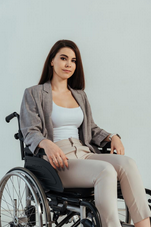
\includegraphics[width=0.5\textwidth]{Imagenes/Personas/Isabel.png}
\end{minipage}

\textbf{Background personal} \\

Isabel es una psicóloga comprometida con la mejora de la calidad de vida de las personas con discapacidad. \textit{Tiene una 
discapacidad física desde su nacimiento} que afecta su movilidad y requiere el uso de una silla de ruedas. Actualmente
\textit{vive en una pequeña urbanización a las afueras de Barcelona}. \\

Su familia vive en un pequeño pueblo de Huesca, por lo que \textit{siempre que puede se desplaza para verlos}. Muchas veces 
tiene el problema de la falta de autobuses que conectan con el pueblo, por lo que \textit{utiliza Omio, que realiza el trayecto
por ella, indicándole los transbordos que tiene que realizar y facilitándole la ayuda que necesita en todo momento}. \\

Ha asistido a varios cursos y conferencias relacionados con la psicología y la discapacidad, lo que la ha llevado a 
\textit{planear viajes a diferentes ciudades para participar en eventos}. Utiliza comparadores de viaje para encontrar opciones 
que se adapten a sus necesidades específicas, como hoteles con habitaciones adaptadas y \textit{vuelos con asistencia en el 
aeropuerto}. \textit{Algunos de los comparadores que usa no tienen opción de solicitar ayuda en caso de que tengas dudas, por lo que si
tiene algún problema no puede contactar con nadie}. Antes de realizar la reserva, ella sabe las distintas compañías y empresas que te lo suelen proporcionar. \\

Aparte de su trabajo, Isabel es una apasionada de la pintura y trata de visitar galerías y estudios de artistas en cada 
destino que visita. Isabel también es miembro activo de grupos de apoyo para personas con discapacidad en su ciudad. \textit{Allí 
es donde comparte experiencias y ofrece apoyo a otros miembros, por ejemplo a los jóvenes con discapacidad, para fomentar 
su independencia y autoestima}. Viaja a menudo con su mejor amiga, Carmen, quien la ha apoyado en su viaje de empoderamiento 
y ha aprendido mucho sobre la discapacidad en el proceso también.

\subsection{Validación de las personas}
Tras revisar las personas obtenidas en el paso anterior, se ha
comprobado que contengan toda la información relevante que sacamos de los factoides,
variables y patrones de comportamiento. También hemos comprobado que todo coincida con los esqueletos de personas. Hemos podido comprobar que en el viajero con discapacidad, en la persona faltaba el factoide de: “Les parece complicado pedir ayuda dentro de las páginas de los comparadores”

Finalmente, el resultado obtenido han sido tres perfiles tal que sus hobbies, background y
objetivos parten de los conocimientos que tenemos acerca de los viajeros que utilizan comparadores, viajeros que no utilizan comparadores, viajeros con discapacidad.

\subsection{Tipos de personas}
\begin{itemize}
    \item \textbf{Persona Primaria} - \textit{Marta González Torres (Viajero que usa comparadores de viajes)} $\rightarrow$ Representa al tipo de usuario consumidor de comparadores de viajes. Se tratan de usuarios que utilizan activamente las funcionalidades de los comparadores con el objetivo de ahorrar lo máximo posible en los transportes para sus viajes.
    \item \textbf{Persona Secundaria} - \textit{Isabel García Rodríguez (Viajero con discapacidad)} $\rightarrow$ Representa al tipo de usuario consumidor o no consumidor de comparadores de viajes que tienen una necesidad añadida o distinta al resto de usuarios. 
    Generalmente usuarios que aparte de la interfaz ya creada necesitaran de una pequeña adaptación visual o sensorial para poder sacar el máximo provecho a la aplicación.
    \item \textbf{Persona Suplementaria} - \textit{Juan Martínez Diaz (Viajero que no usa comparadores de viajes)} $\rightarrow$ Representa al tipo de usuario que no suele usar comparadores de viajes de forma habitual. Buscan experiencias espontáneas y diversas en sus viajes. No es recurrente al uso de comparadores debido a que prefieren contactar con una agencia o familiares que les den todo el trabajo hecho. Pero cuando utilizan los comparadores, las interfaces creadas para satisfacer las necesidades de las personas primarias y secundarias son más que suficientes para satisfacer las suyas.
\end{itemize}